\documentclass[a4paper,12pt]{article}

%% Definitioner för LIPS-dokument

\usepackage[english]{babel}
\usepackage[utf8]{inputenc}
\usepackage[T1]{fontenc}
\usepackage{times}
\usepackage{ifthen}

\usepackage[margin=25mm]{geometry}

\usepackage{fancyhdr}
\pagestyle{fancy}
\lhead{}
\chead{\textbf{\LIPSprojekttitel}}
\rhead{\textbf{\textsl{LiTH}}\\\textbf{\LIPSdatum}}
\lfoot{\textbf{\LIPSkursnamn}\\\textbf{\LIPSdokumentansvarig}}
\cfoot{\textbf{\LIPSprojektgrupp}\\\textbf{\LIPSgruppepost}}
\rfoot{\textbf{\textsc{Lip}s}\\\textbf{Page~\thepage}}

\setlength{\parindent}{0pt}
\setlength{\parskip}{1ex plus 0.5ex minus 0.2ex}


\newcommand{\twodigit}[1]{\ifthenelse{#1<10}{0}{}{#1}}
\newcommand{\dagensdatum}{\number\year-\twodigit{\number\month}-\twodigit{\number\day}}

%%  Redefinitions of commands containing @
\makeatletter
\makeatother

\newcommand{\LIPStitelsida}{%
{\ }\vspace{45mm}
\begin{center}
  \textbf{\Huge \LIPSdokumenttyp}
\end{center}
\begin{center}
  {\Large Editor: \LIPSredaktor}
\end{center}
\begin{center}
  {\Large \textbf{Version \LIPSversion}}
\end{center}
\vfill
\begin{center}
  {\large Status}\\[1.5ex]
  \begin{tabular}{|*{3}{p{40mm}|}}
    \hline
    Reviewed & \LIPSgranskare & \LIPSgranskatdatum \\
    \hline
    Approved & \LIPSgodkannare & \LIPSgodkantdatum \\
    \hline
  \end{tabular}
\end{center}
\newpage
}


\newenvironment{LIPSprojektidentitet}{%
{\ }\vspace{45mm}
\begin{center}
  {\Large PROJECT IDENTITY}\\[0.5ex]
  {\small
  \LIPSartaltermin, \LIPSprojektgrupp\\
  Linköping Institute of Technology, IFM
  }
\end{center}
\begin{center}
  {\small Group members}\\
%  \begin{tabular}{|p{30mm}|p{40mm}|p{35mm}|p{45mm}|}
  \begin{tabular}{|l|l|p{25mm}|l|}
    \hline
    \textbf{Name} & \textbf{Responsibility} & \textbf{Phone} & \textbf{E-mail} \\
    \hline
}%
{%
    \hline
  \end{tabular}
\end{center}
\begin{center}
  {\small
%    \textbf{E-mail for the group}: \LIPSgruppepost\\
%    \textbf{Webpage}: \LIPSgrupphemsida\\[1ex]
    \textbf{Customer}: \LIPSkund\\
    \textbf{Customer contact}: \LIPSkundkontakt\\
    \textbf{Sponsor/Course leader}: \LIPSkursansvarig\\
    \textbf{Supervisors/Experts}: \LIPShandledare\\
  }
\end{center}
\newpage
}
\newcommand{\LIPSgruppmedlem}[4]{\hline {#1} & {#2} & {#3} & {#4} \\}



\newenvironment{LIPSdokumenthistorik}{%
\begin{center}
  Version log\\[1ex]
  \begin{small}
    \begin{tabular}{|l|l|p{60mm}|l|l|}
      \hline
      \textbf{Version} & \textbf{Date} & \textbf{Performed changes} & \textbf{Performed by} & \textbf{Reviewed} \\
      }%
    {%
      \hline
    \end{tabular}
  \end{small}
\end{center}
}
\newcommand{\LIPSversionsinfo}[5]{\hline {#1} & {#2} & {#3} & {#4} & {#5} \\}

\newcounter{LIPSkravnummer}
\newcounter{LIPSunderkravnummer}[LIPSkravnummer]
\newenvironment{LIPSkravlista}{%
  \begin{tabular}{|p{25mm}|p{25mm}|p{72mm}|p{18mm}|}
    }%
  {%
    \hline
  \end{tabular}
}
\newcommand{\LIPSmilstolpe}[3]{\hline {#1} & {#2} & {#3} \\}
\newcounter{LIPSaktivitetsnummer}
\newcommand{\LIPSaktivitet}[3]{\hline\stepcounter{LIPSaktivitetsnummer}\textbf{\arabic{LIPSaktivitetsnummer}} & {#1} & {#2} & {#3} \\}

\newcommand{\LIPSkrav}[3]{\hline\stepcounter{LIPSkravnummer}\textbf{Krav nr \arabic{LIPSkravnummer}} & \textbf{{#1}} & {#2} & \textbf{{#3}} \\}
\newcommand{\LIPSunderkrav}[3]{\hline\stepcounter{LIPSunderkravnummer}\textbf{Requirement nr. \arabic{LIPSkravnummer}\Alph{LIPSunderkravnummer}} & \textbf{{#1}} & {#2} & \textbf{{#3}} \\}

\newcommand{\LIPSleverans}[4]{\hline {#1} & {#2} & {#3} & {#4} \\}


%%% Local Variables: 
%%% mode: latex
%%% TeX-master: "kravspec_mall"
%%% End: 

\usepackage{graphicx}
\usepackage{epstopdf}
\usepackage{gensymb}
\usepackage{longtable}


\newcommand{\LIPSartaltermin}{2013/HT}
\newcommand{\LIPSkursnamn}{TFYA50}

\newcommand{\LIPSprojekttitel}{Computational Physics}

\newcommand{\LIPSprojektgrupp}{Group 2}
\newcommand{\LIPSgruppepost}{}
\newcommand{\LIPSgrupphemsida}{}

\newcommand{\LIPSdokumentansvarig}{Björn Lindström}

\newcommand{\LIPSkund}{IFM at Linköping University - 581 00 Linköping - customer phone: 013-28 10 00 - fax: 013-13 75 68 - info@ifm.liu.se}
\newcommand{\LIPSkundkontakt}{Valeriu Chirita - 013-28 12 89 - vio@ifm.liu.se - office: G305}
\newcommand{\LIPSkursansvarig}{Valeriu Chirita - 013-28 12 89 - vio@ifm.liu.se - office: G305}
\newcommand{\LIPShandledare}{Daniel Edström - 013-28 66 93 - daned@ifm.liu.se - office: G432\\Davide Sangiovanni - 013-28 26 23 - davsan@ifm.liu.se - office: G426}


\newcommand{\LIPSdokumenttyp}{Project plan}
\newcommand{\LIPSredaktor}{Simon Wallin}
\newcommand{\LIPSversion}{0.1}
\newcommand{\LIPSdatum}{\dagensdatum}

\newcommand{\LIPSgranskare}{Björn Lindström}
\newcommand{\LIPSgranskatdatum}{\dagensdatum}
\newcommand{\LIPSgodkannare}{Valeriu Chirita}
\newcommand{\LIPSgodkantdatum}{}

\begin{document}

\LIPStitelsida

%% Argument till \LIPSgruppmedlem: namn, roll i gruppen, telefonnummer, epost
\begin{LIPSprojektidentitet}
	\LIPSgruppmedlem{Simon Wallin}{Project leader (PL)}{0762-30 06 65}{simwa252@student.liu.se}
	\LIPSgruppmedlem{Björn Lindström}{Documents (DOC)}{0735-33 55 98}{bjoli010@student.liu.se}
	\LIPSgruppmedlem{Johan Jönsson}{Code implementation (CI)}{0738-30 57 58}{johjo939@student.liu.se}
	\LIPSgruppmedlem{Fran\c{c}ois Vrel}{Code design (CD)}{0765-80 96 64}{fravr827@student.liu.se}
	\LIPSgruppmedlem{Mohammed Rashed}{Program operation (PO)}{0739-58 04 98}{mohra020@student.liu.se}
	\LIPSgruppmedlem{Simon Larsson}{Code test (CT)}{0707-31 16 46}{simla804@student.liu.se}
\end{LIPSprojektidentitet}

\tableofcontents{}
\newpage

%% Argument till \LIPSversionsinfo: versionsnummer, datum, ändringar, utfört av, granskat av
\addcontentsline{toc}{section}{Version log}
\begin{LIPSdokumenthistorik}
  \LIPSversionsinfo{0.1}{}{}{}{}
\end{LIPSdokumenthistorik}
\newpage

\section{Who is the customer}
\section{An overview of the system}
\section{Plan for the project phases}

\subsection{Before}
In the ''before'' phase focus will be on planning the work to be done during
the two remaining phases. In addition to planning the project there will also
be some education to prepare the group members for the project, i.e.
laborations, lectures and information regarding what tools will be used during
the project.

\subsection{During}
During the ''during'' phase, focus will be on writing the code for the
MD simulation and writing the documentation to be handed in with the finished
program.

\subsection{After}                     
After the delivery of the finished MD simulation software the
client will determine whether or not the finished product satisfies the
requirements specified in the Project Requirements document. Afterwards
every group member will fill out an evaluation which will be handed in to the sponsor.

\section{Organization plan} %%SW
This part aims to give an overview of the organizational parts of the project, first for the whole project and then for the customer, group and last responsibilities.
\subsection{Organization plan for the whole project}
The distribution of responsibility and an overview of the communication are given in figure\ref{FlowOrg}.
\begin{figure}[h]
	\centering
		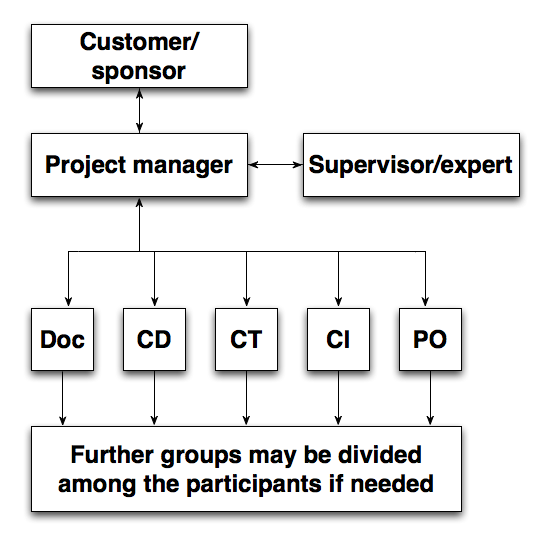
\includegraphics[width=0.7\textwidth]{Images/FlowChart_Org.png}
		\caption{Overview of responsibility and communication}
		\label{FlowOrg}
\end{figure}
The contact between the customer and the group goes mainly through the project leader. Every group member has his own area of responsibility and it is the PM:s responsibility to make sure that all the group members work toward the same goal, that no tollgates/milestones are missed, and that there is at least one group member responsible for every task. The PM also divides the project group into smaller groups throughout the project so that the workload is evenly distributed over all the members. The experts may be consulted when required, to solve parts of the project or when problems occur.
\subsection{The customer organization}
The customer is responsible for approving the tollgates and should be informed/consulted when the milestones are reached.
\subsection{Conditions for the cooperation in the project group}
There is a letter of agreement that will be discussed and developed from the template in Appendix \ref{LetterOA}. The finished group contract will then be signed by all members.
\subsection{Definition of work contents and responsibilities}
\begin{tabular}{|p{16mm}|p{31mm}|p{100mm}|}
        	\LIPSmilstolpe{\textbf{Name}}{\textbf{Responsibility}}{\textbf{Comment}}
	\LIPSmilstolpe{Simon Wallin}{Project Manager}{Responsible for the general process of the project and that the TG/MS as well as requirements are met. Also responsible for keeping track of time logging and contact with the customer.}
	\LIPSmilstolpe{Björn Lindström}{Documents (Doc)}{Responsible for a uniformed documentation and keeping track of meeting protocols.}
	\LIPSmilstolpe{Francois Vrel}{Code Design (CD)}{Has the main responsibility for the design of the code.}
	\LIPSmilstolpe{Simon Larsson}{Code Test (CT)}{Responsible for putting together a test plan and making sure that this is used throughout the project.}
	\LIPSmilstolpe{Johan Jönsson}{Code Implementation (CI)}{Has the main responsibility for making sure that all the code is implemented and also in the best possible manner.a}
	\LIPSmilstolpe{Mohammed Rashed}{Program Operation (PO)}{Has the main responsibility to make sure that the program operates as intended.}
\hline
\end{tabular}

\section{Document plan}
The purpose of the documentation is to keep all parties up-to-date regarding the progress of the project, as well as helping the project group in its’ work.\\
\begin{tabular}{|p{40mm}|p{20mm}|p{50mm}|p{23mm}|}
\LIPSleverans{\textbf{Document}}{\textbf{Author / Approved by}}{\textbf{Purpose}}{\textbf{Due date}}
\LIPSleverans{Project directives}{PM/SP}{Definition of all requirements}{2013-09-20}
\LIPSleverans{Proejct Plan}{PM/SP}{Description of how the project will be executed}{2013-09-27}
\LIPSleverans{Time Plan}{PM/SP}{Specification of how the time will be distributed}{?}
\LIPSleverans{Main Subroutines Design}{CD/SP}{Complete description of the main subroutines (integrators, force calculation)}{2013-10-11}
\LIPSleverans{MD Code Design}{CD/SP}{Complete description of the MD code}{2013-10-18/25}
\LIPSleverans{Program Description}{PO/PM}{General description of the program, including capabilities and how to operate}{?}
\LIPSleverans{Results}{CT/PM}{Results of processes/properties}{?}
\LIPSleverans{Analysis}{/PM}{Analysis results}{?}
\LIPSleverans{Comparison}{/PM}{Comparison of results with experiments}{?}
\LIPSleverans{Final Report}{DOC/SP}{Final report containing the documents Program Description, Results, Analysis and Comparison}{2013-12-13/20}
\LIPSleverans{Time Report(?)}{PM/SP}{Specification of how time was spent}{?}
\LIPSleverans{Reflection}{individual/SP}{Evaluation of one’s own work, as well as the course and the project}{?}
\hline
\end{tabular}
\section{Development method}

Development Method
There are many development methods, and we prefer the conventional method it is Waterfall. The waterfall model can work if everything goes to plan, but in a complex project things rarely do. The core of the problem is the reliance on getting the specification perfect before attempting to it.

\begin{figure}[h]
	\centering
	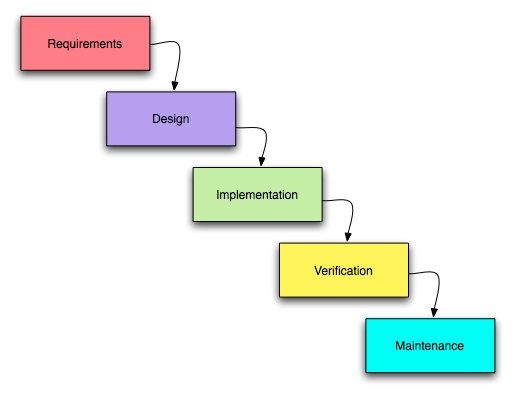
\includegraphics[width=0.5\textwidth]{Images/development_method_waterfall_model.png}
	\caption{Waterfall model}
	\label{Waterfall}
\end{figure}

The waterfall model shows a process, where developers are to follow these phases in order:
\begin{enumerate}
\item Requirements specification (Requirements analysis)
\item Software design
\item Implementation and Integration
\item Testing (or Validation)
\item Deployment (or Installation)
\item Maintenance
\end{enumerate}

\begin{figure}[h]
	\centering
	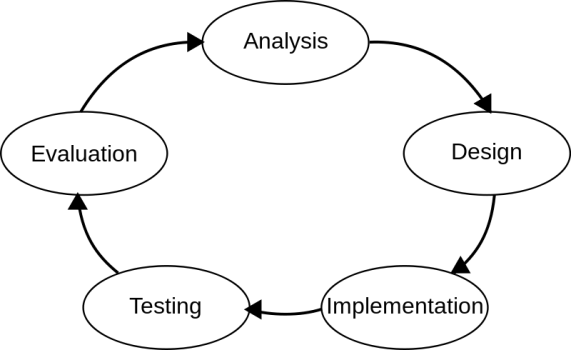
\includegraphics[width=0.5\textwidth]{Images/development_method_software_development_cycle.png}
	\caption{Software Development cycle l}
	\label{cyclel}
\end{figure}



Software Development cycle 
\section{Training plan}

\subsection{Group training}
For all members of the project group to be able to contribute equally to the project, there might be some small lessons or training in the different tools that will be used, such as C/C++, git, the graphics library OpenGL etc. The group will also be given lectures and some training in MD simulations.

In the course, TFYA50, that the project is a part of there will also be lectures in entrepeneurship, some case studies and an exam. All given by Magnus Klofsten from IEI.

The MD laborations are compulsory for all group members and are given to prepare the group for the project.

\subsection{Client training}
All information necessary for the client to use the finished product will be given in the technical documentation written during the project. No other training for the client is necessary.

\section{Report plan}
The time that each group member spend on the project will be logged and the PL will then report this to the customer. Each member is responsible to log how much time he has spend and PL is responsible for reporting this to the costumer.
\section{Meeting plan}
All meetings shall be advertised at least 48 hours before the start of the meeting. Meetings may occur over lunch or when best fitted for the group. A weekly time slot for meetings will be decided by the group and all members shall keep this time slot free every week. However if there is nothing of importance to discuss reported 48 hours prior to the meeting start, it may be canceled. When a meeting is needed and it is not possible to advertise this 48 hours in advance the rules of attendance might be relaxed.
\subsection{Group meetings}
For every group meeting an agenda will be sent out prior to the start of the meeting. If the meeting is not at the weekly meeting time it needs to be addressed 48 hours prior to the meeting start via either email or SMS. The attendance is compulsory, with the exception of reasonable excuses such as sickness.
\subsection{Customer meetings}
For the customer meetings where the whole group is supposed to be present attendance is compulsory. If a group member cannot attend the meeting it should be postponed until the whole group can attend.

\section{Resource plan}
\section{Milestones and tollgates}
\section{Activities}

\begin{longtable}{|p{7mm}|p{90mm}|p{23mm}|p{23mm}|}
	\LIPSleverans{\textbf{Nr}}{\textbf{Description}}{\textbf{Depends on}}{}
%	\LIPSaktivitet{}{}{}
	\LIPSaktivitet{Design of potential and force calculations}{}{}
	\LIPSaktivitet{Design of numerical integrator}{}{}
	\LIPSaktivitet{Design of MD setup}{}{}	
	\LIPSaktivitet{Design of neighbor list}{}{}
	\LIPSaktivitet{Design of average properties}{}{}
	\LIPSaktivitet{Design of instant properties}{}{}
	\LIPSaktivitet{Design of I/O handling}{}{}
	\LIPSaktivitet{Layout of graphical user interface}{1,3,5,6}{}
	\LIPSaktivitet{Code for potential and force calculations}{1}{}
	\LIPSaktivitet{Code for numerical integrator}{2}{}
	\LIPSaktivitet{Code for MD setup}{3}{}
	\LIPSaktivitet{Code for neighbor list}{4}{}
	\LIPSaktivitet{Code for average properties}{5}{}
	\LIPSaktivitet{Code for instant properties}{6}{}
	\LIPSaktivitet{Code for I/O handling}{7}{}
	\LIPSaktivitet{Code for graphical user interface}{8}{}


	\LIPSaktivitet{Integration of code for different modules}{}{}
	\LIPSaktivitet{Testing of entire program}{}{}
	\LIPSaktivitet{Verification of modules and entire program}{}{}
	\LIPSaktivitet{Research parameters and materials}{}{}
	\LIPSaktivitet{Simulations for final report}{}{}
	\LIPSaktivitet{Analysis of simulations}{}{}
	\LIPSaktivitet{Completion of technical documentation}{}{}
	\LIPSaktivitet{Completion of user's manual}{}{}
	\LIPSaktivitet{Preparation of final presentation}{}{}
	\LIPSaktivitet{Evaluation of project}{}{}

\hline
\end{longtable}

\section{Timetable}
\section{Quality plan}
Two different methods will be used to guarantee the quality of the product and documentation, tests and reviews. Tests regards all necessary documentation for the project. Furthermore tests will continuously be made during the project make sure that every part of the MD programme works as it should.

\subsection{Reviews}

Each new version of the documentation shall be reviewed by at least one group member before it can be regarded as ready for handing in. If nothing else has been agreed, the group member with responsibility for the documentation (Björn Lindström) is responsible for making sure that the document is being reviewed. The purpose of the reviewing is to make sure that the document contains all necessary parts and that no major language or layout errors have been made.

\subsection{Test plan}

Several tests will be made during the project to make sure that the result of the work fulfil the requirements. The group member with responsibility for code test (Simon Larsson) is responsible for planning and performing of the tests, and for creating a test plan that describes how to perform the tests and which requirements that has to be fulfilled to pass the test.



\section{Priorities}
The group shall first of all aim to make sure that all requirements with high/mandatory priority in the requirement specification are working sufficiently. In case of time shortage or other unexpected obstacles, the customer shall be contacted for a discussion about the requirement’s necessity and potential changes in the requirement specification. Another possible reason for discussing a requirement with the customer could be that the group considers that a disproportionate amount of time is needed to fulfil a relatively unimportant requirement, such that it affects other activities and project goals negatively.

\section{Project Closing}
In week 50 the finished program, along with the technical documenatation and the
user's manual will be handed in to the customer. That same week a short
presentation of the finished program and some of the finished simulations will
be given. The week after, week 51, the group members will individually complete 
an evaluation of the project and hand it in to the sponsor.


% \begin{tabular}{|p{43mm}|p{15mm}|p{70mm}|p{23mm}|}
% \LIPSleverans{\textbf{Leverans}}{\textbf{Ansvarig / Godkänns av}}{\textbf{Syfte}}{\textbf{Färdig-datum}}
% \LIPSleverans{Första version av Projektplan, tidplan och systemskiss}{Simon L / Tomas}{Beskriver hur projektet ska utföras och ger en handvisning till hur roboten ska fungera}{15/2-2012}
% \LIPSleverans{Slutgiltig version av Projektplan, tidplan och systemskiss}{Simon L / Tomas}{Beskriver hur projektet ska utföras och ger en handvisning till hur konstruktionen av roboten ska ske}{23/2-2012}
% \LIPSleverans{Första version av designspecifikation}{Johan / Olov}{Visar mer detaljerat hur konstruktionen av roboten ska ske}{13/3-2012}
% \LIPSleverans{Slutgiltig version av designspecifikation}{Simon L / Olov}{Visar mer detaljerat hur konstruktionen av roboten ska ske}{16/3-2012}
% \LIPSleverans{Tidrapporter och uppdaterad tidplan}{Simon L / Tomas}{Visar hur tidfördelningen mellan de olika aktiviteterna har gått under den senaste tidsperioden, samt hur projektgruppen tänkt lägga upp sitt framtida arbete}{12/3, 19/3, 26/3, 2/4, 16/4, 23/4, 30/4, 7/5, 14/5, 21/5}
% \LIPSleverans{Statusrapport för projektet}{Simon L / Tomas}{Ger en bild av projektgruppens nuvarande status i förhållande till tidigare planering}{Vid begäran}
% \LIPSleverans{Teknisk dokumentation och användaranvisning}{Gustav / Tomas}{Ger en detaljerad bild över hur systemet fungerar, information om användargränssnit och beskrivning hur roboten används}{Tre arbetsdagar innan redovisningen vecka 20}
% \LIPSleverans{Muntlig presetation och demonstration}{Simon L / Tomas}{Slutleveransen som består av en 15-20 minuter lång presentation av robotens specifikationer och funktioner}{Vecka 20}
% \LIPSleverans{Leverans av robot}{Markus / Tomas}{En robot som uppfyller ställda krav levereras till beställaren}{vecka 20, 2012}
% \LIPSleverans{Efterstudie}{Simon L / (delges senare)}{Projektgruppen sammanställer här sina erfarenheter från projektarbetet och lämnar synpunkter på hur projektkursen skulle kunna förändras}{1/6-2012}
% \hline
% \end{tabular}




% \begin{tabular}{|p{16mm}|p{31mm}|p{100mm}|}
%         	\LIPSmilstolpe{\textbf{Namn}}{\textbf{Ansvarsområde}}{\textbf{Kommentar}}
% 	\LIPSmilstolpe{Simon L}{Projektledare}{Ansvarar för att projektgruppens sammanlagda arbete går framåt mot uppsatta mål. Uppdaterar tidsplanen och skickar in tidrapport enl. överenskommelse med beställaren}
% 	\LIPSmilstolpe{Mattias}{Dokumentansvarig}{Ansvarar för alla dokument och möteshandlingar}
% 	\LIPSmilstolpe{Gustav}{Ansvarig för reglersystem}{Huvudansvarig för robotens styr-och reglersystem}
% 	\LIPSmilstolpe{Johan}{Mjukvaruansvarig}{Ansvarar för framtagande och optimering av all programmeringskod i projektet.}
% 	\LIPSmilstolpe{Tobias}{Hårdvaruansvarig}{Ansvarar för konstruktion av nödvändig hårdvara}
% 	\LIPSmilstolpe{Simon W}{Testansvarig}{Ansvarig för att upprätta en testplan och kontinuerligt genomföra tester enligt denna}
% \hline
% \end{tabular}

% \begin{tabular}{|p{40mm}|p{20mm}|p{50mm}|p{23mm}|}
% \LIPSleverans{\textbf{Dokument}}{\textbf{Ansvarig / Godkänns av}}{\textbf{Syfte}}{\textbf{Färdig-datum}}
% \LIPSleverans{Kravspecifikation}{Simon L / Tomas}{Definierar kraven som ställs på projektet}{2/2-2012}
% \LIPSleverans{Projektplan, första inlämningnen}{Markus / Tomas}{Beskriver hur projektet ska utföras.}{15/2-2012}
% \LIPSleverans{Systemskiss, första inlämningnen}{Markus / Tomas}{Beskriver hur systemet ska byggas upp}{15/2-2012}
% \LIPSleverans{Tidplan, första inlämningnen}{Markus / Tomas}{Listar aktiviteternas budgeterade tidsåtgång.}{15/2-2012}
% \LIPSleverans{Projektplan, slutgiltig inlämning}{Simon L / Tomas}{Beskriver hur projektet ska utföras.}{23/2-2012}
% \LIPSleverans{Systemskiss, slutgiltig inlämning}{Simon L / Tomas}{Beskriver hur systemet ska byggas upp}{23/2-2012}
% \LIPSleverans{Tidplan, slutgiltig inlämning}{Simon L / Tomas}{Listar aktiviteternas budgeterade tidsåtgång.}{23/2-2012}
% \LIPSleverans{Designspecifikation, första inlämningen}{Johan / Olov}{Visar mer detaljerat hur konstruktionen av roboten ska ske}{13/3-2012}
% \LIPSleverans{Designspecifikation, slutlig inlämning}{Simon L / Olov}{Visar mer detaljerat hur konstruktionen av roboten ska ske. Version 1.0 och högre skickas till Tomas}{16/3-2012}
% \LIPSleverans{Tidrapporter och uppdaterad tidplan}{Markus / Tomas}{Visar budgeterad och spenderad tid, uppdelad på de olika aktiviteterna}{Måndagar varje vecka, med start 12/3 och slut 21/5-2012 (undantaget 9/4)}
% \LIPSleverans{Statusrapport för projektet}{Simon L / Tomas}{Dokumentet ska översiktligt sammanfatta hur projektet fortskrider.}{Vid begäran}
% \LIPSleverans{Teknisk dokumentation}{Gustav / Tomas}{Beskriver i detalj systemets uppbyggnad}{Tre arbetsdagar innan redovisningen, vecka 20}
% \LIPSleverans{Användaranvisning}{Mattias / Tomas}{Beskriver hur produkten används och dess olika funktioner.}{Tre arbetsdagar innan redovisningen, vecka 20}
% \LIPSleverans{Efterstudiedokument}{Simon L / (delges senare)}{Dokumenterar gruppens reflektioner över projektet och hur det har genomförts}{1/6-2012}
% \hline
% \end{tabular}

%%\section{Utvecklingsmetodik}

% \begin{tabular}{|p{7mm}|p{117mm}|p{23mm}|}
%         	\LIPSmilstolpe{\textbf{Nr}}{\textbf{Beskrivning}}{\textbf{Datum}}
% 	\LIPSmilstolpe{1}{Designspecifikationen accepterad av handledaren}{2012-03-16}
% 	\LIPSmilstolpe{2}{Bussen fungerar som den ska}{2012-03-23}
% 	\LIPSmilstolpe{3}{Data och mätvärden skickas via komunikationsenheten}{2012-04-30}
% 	\LIPSmilstolpe{4}{Roboten kan upptäcka korsningar}{2012-04-19}
% 	\LIPSmilstolpe{5}{Korrekt sensorinfo visas på PCn}{2012-04-20}
% 	\LIPSmilstolpe{6}{Motorn regleras autonomt utifrån sensorvärdena}{2012-04-27}
% 	\LIPSmilstolpe{7}{Styrkommandon utförs korrekt}{2012-05-04}
% \hline
% \end{tabular}

% \begin{tabular}{|p{7mm}|p{117mm}|p{23mm}|}
%         	\LIPSmilstolpe{\textbf{BP}}{\textbf{Beskrivning}}{\textbf{Datum}}
% 	\LIPSmilstolpe{BP0}{Godkännande av projektdirektiv, beslut att starta förstudie}{2012-01-20}
% 	\LIPSmilstolpe{BP1}{Godkännande av kravspecifikation, beslut att starta förberedelsefasen}{2012-02-02}
% 	\LIPSmilstolpe{BP2}{Godkännande av projektplanering, beslut att starta utförandefasen}{2012-02-23}
% 	\LIPSmilstolpe{BP3}{Godkännande av designspecifikation, beslut att fortsätta utförandefasen}{2012-03-16}
% 	\LIPSmilstolpe{BP4}{Ej specifierad}{-}
% 	\LIPSmilstolpe{BP5}{Godkännande av produktens funktionalitet, beslut att leverera}{vecka 19}
% 	\LIPSmilstolpe{BP6}{Godkännande av leverans, beslut att upplösa projektgruppen}{2012-06-01}
% \hline
% \end{tabular}

% \begin{longtable}{|p{7mm}|p{90mm}|p{23mm}|p{23mm}|}
% 	\LIPSleverans{\textbf{Nr}}{\textbf{Beskrivning}}{\textbf{Beroende av aktivitet nr}}{\textbf{Beräknad tid (h)}} 
% \LIPSaktivitet{Färdigställande av
% designspec}{}{44} 
% %% SENSOR
% 	\LIPSaktivitet{Omvandling av analoga signaler till
% digitala sådana}{}{12} 
% 	\LIPSaktivitet{Trösklande av
% sensorvärden}{2}{4} 
% 	\LIPSaktivitet{Hitt skillnaden mellan önskade och
% aktuella värden}{3}{4} 
% 	\LIPSaktivitet{Skicka skilnaden till styrenheten (via
% kommunikationsenheten)}{4 \& 10}{14} 
% 	\LIPSaktivitet{Skicka avstånd i cm till display- och
% kommunikationsenheten}{2 \& 10}{12} 
% 	\LIPSaktivitet{Upptäck
% riktningsmarkeringar}{1 \& 2}{20} 
% 	\LIPSaktivitet{Hantera
% riktningsmarkeringar}{6}{20} 
% 	\LIPSaktivitet{Upptäck korsningar}{2 \&
% 3}{20} 
% %% KOMMUNIKATION
% 	\LIPSaktivitet{Ordna master som sköter
% buss}{}{50} 
% 	\LIPSaktivitet{Skicka styrinfo till
% pc}{15 \& 23 \& 10}{15} 
% 	\LIPSaktivitet{Skicka sensorinfo till
% pc}{5 \& 15 \& 23}{15} 
% 	\LIPSaktivitet{Ta emot styrkommandon från
% pc}{15 \& 23}{15} 
% 	\LIPSaktivitet{Skicka styrkommando till styrenhet
% från kommunikqtionsenhet}{10}{15} 
% 	\LIPSaktivitet{Fixa blåtand i
% kommunikationsenhet}{}{25} 
% %% STYRENHET
% 	\LIPSaktivitet{Ta emot sensorvärden
% (Styrenhet)}{10 \& 5}{20} 
% 	\LIPSaktivitet{Reglera motorer utifrånsensorvärden}{16 \& 19 \& 22}{40} 
% 	\LIPSaktivitet{Ta emot styrkommandon
% (styrenheten)från kommunikationsenheten}{10 \& 24 \& 14}{20} 
% 	\LIPSaktivitet{Styra motorer (autonomt och manuellt)}{}{40} 
% 	\LIPSaktivitet{Skicka styrinfo till
% kommunikationsenheten från
% styrenheten}{10}{20} 
% 	\LIPSaktivitet{Hantera
% specialkommandon}{8 \& 19}{30}
% 	\LIPSaktivitet{Regulator}{5}{30} 
% %% PC 
% 	\LIPSaktivitet{Fixa blåtand i
% pc}{}{25} 
% 	\LIPSaktivitet{Hämta och skicka styrkommandon från
% pc till kommunikationsenheten (Mjukvara)}{15 \& 23}{30} 
% 	\LIPSaktivitet{Ta emot styrinfo i PC från
% kommunikationsenheten}{15 \& 23 \& 20}{20} 
% 	\LIPSaktivitet{Ta emot sensorinfo}{15 \& 23 \&
% 6}{20} 
% 	\LIPSaktivitet{Visa styrinfo på
% skärm}{25}{2} 
% 	\LIPSaktivitet{Visa sensorinfo på
% skärm}{26}{2} 
% 	\LIPSaktivitet{Ordna gränssnitt på
% pc}{}{15} 
% %% MONTERING OCH TEST
% 	\LIPSaktivitet{Montering av
% avståndssensorer}{}{10} 
% 	\LIPSaktivitet{Montering av
% linjesensorer}{}{10}
% 	\LIPSaktivitet{Montering}{30 \&
% 31}{20} 
% 	\LIPSaktivitet{Utför styrkommandon}{18 \&
% 21}{30} 
% 	\LIPSaktivitet{Test av hela systemet}{2-33 \& (35)}{35} 
% 	\LIPSaktivitet{Kalibrering av
% sensorer}{}{20}
% 	\LIPSaktivitet{Planering och utförande av tester}{}{10}
% 	\LIPSaktivitet{Test av bussen}{}{10}
% 	\LIPSaktivitet{Test av kommunikationsenheten}{}{10}
% 	\LIPSaktivitet{Test av sensorenheten}{}{10}
% 	\LIPSaktivitet{Test av styrenheten}{}{10}
% %% EFTERARBETE OCH DOKUMENTATION
% 	\LIPSaktivitet{Sammanställa och granska
% teknisk dokumentation}{samtliga}{20} 
% 	\LIPSaktivitet{Sammanställa och granska
% Användarmanual}{37}{20} 
% 	\LIPSaktivitet{Förbereda
% redovisning}{38}{15} 
% 	\LIPSaktivitet{Tidsloggning (ska ske
% kontinuerligt)}{}{20} 
% 	\LIPSaktivitet{Efterstudie}{39}{15}  
% 	\LIPSaktivitet{Rest / Reservtid}{}{46}
% 	\LIPSaktivitet{Möten}{}{70} 
% 
% \hline
% \end{longtable}
\newpage
\appendix

\newpage


\addcontentsline{toc}{section}{References}
\begin{thebibliography}{99}
\bibitem{lipskompendiet}\textit{Projektmodellen LIPS - } Svensson, Tomas
\\Studentlitteratur, 2011.
\end{thebibliography}

\end{document} 

%%% Local Variables: 
%%% mode: latex
%%% TeX-master: t
%%% End: 

